\documentclass{scrartcl}

\usepackage{multirow}

\usepackage{listings}
\lstset{basicstyle=\footnotesize\ttfamily}

\usepackage{pgf}
\usepackage{tikz}
\usetikzlibrary{arrows,positioning,graphs,shapes,shapes.geometric}
%\usetikzlibrary{}

\title{MUSTE server protocol}
\author{Herbert Lange}
\date{Document version 0.0.1}
\begin{document}
\maketitle

\section{Design principles}

\begin{itemize}
\item stateful - authentication happens once
\item unidirectional - client sends request, server answers
\end{itemize}

\section{Message format}

\begin{itemize}
\item Client messages (CM) are messages from the client sent to the server

  \begin{tabular}{llp{0.6\textwidth}}
    Message Name                      & Valid Responses   & Description \\
    \hline
    \multirow{2}{*}{CMLoginRequest}   & SMLoginSuccess & \multirow{2}{*}{Send login request} \\
                                      & SMLoginFail \\
    \hline
    \multirow{2}{*}{CMMOTDRequest}    & SMMOTDResponse    & \multirow{2}{0.6\textwidth}{Request a Message-of-the-day, e.g. the user survey from the server} \\
                                      & SMSessionInvalid \\
    \hline
    \multirow{3}{*}{CMDataResponse}   & SMDataReceived    & \multirow{3}{*}{Send result of the survey} \\
                                      & SMDataInvalid \\
                                      & SMSessionInvalid \\
    \hline
    \multirow{2}{*}{CMLessonsRequest} & SMLessonsList     & \multirow{2}{*}{Request available lessons} \\
                                      & SMSessionInvalid \\
    \hline
    \multirow{3}{*}{CMLessonInit}     & SMMenuList     & \multirow{3}{*}{Start a new lesson} \\
                                      & SMLessonInvalid \\
                                      & SMSessionInvalid \\
    \hline
    \multirow{3}{*}{CMMenuRequest}    & SMMenuList        & \multirow{3}{*}{Send request for menus} \\
                                      & SMLessonInvalid \\
                                      & SMSessionInvalid \\
    \hline
    CMLogoutRequest                   & SMLogoutResponse & Ends a session \\
    \hline
\end{tabular}

\item Server messages (SM) are messages from the servert sent to a client

  \begin{tabular}{ll}
    Message Name      & Description \\
    \hline
    SMLoginSuccess & Login successful \\
    SMLoginFail     & Login failed \\
    SMMOTDResponse    & A potential html-fragment for a message of the day \\
    SMSessionInvalid  & Invalid Session \\
    SMDataReceived    & Data received \\
    SMDataInvalid     & Invalid data \\
    SMLessonsList     & Lesson listing \\
%    SMLessonStart     & Initial data for a lesson \\
    SMLessonInvalid   & Invalid lesson \\
    SMMenuList        & List of possible menus in a lesson \\
  \end{tabular}

\end{itemize}

\section{Message Datatypes}

General format:
\begin{lstlisting}
  {"message":string, "parameters":object}
\end{lstlisting}
With \texttt{message} field containing the message name and \texttt{parameters} containing (optional) message parameters.

\begin{tabular}{lll}
  Message & Parameters \\
  \hline
  CMLoginRequest &
  \begin{lstlisting}
    {"username":string,"password":string}
  \end{lstlisting} \\
  \hline
  CMMOTDRequest &
  \begin{lstlisting}
    {"token":string}
  \end{lstlisting} \\
  \hline
  CMDataResponse &
  \begin{lstlisting}
    {"token":string,"context":string,
     "data":["field":string,"value":string]}
  \end{lstlisting} & {\bfseries\footnotesize 1} \\
  \hline
  CMLessonsRequest &
  \begin{lstlisting}
    {"token":string}
  \end{lstlisting} \\
  \hline
  CMLessonInit &
  \begin{lstlisting}
    {"token":string,"lesson":string}
  \end{lstlisting} \\
  \hline
  CMMenuRequest &
  \begin{lstlisting}
    {"token":string,"lesson":string,"clicks":number,"time":number,
      "a":{"tree":string,"lang":string},
      "b":{"tree":string,"lang":string}
    }
  \end{lstlisting} \\
  \hline
  CMLogoutRequest &
  \begin{lstlisting}
    {"token":string}
  \end{lstlisting} \\
  \hline
  SMLoginSuccessful &
  \begin{lstlisting}
    {"token":string}
  \end{lstlisting} & {\bfseries\footnotesize 2} \\
  \hline
  SMLoginFail &
  \begin{lstlisting}
    null
  \end{lstlisting} \\
  \hline
  SMMOTDResponse &
  \begin{lstlisting}
    {"filename":string}
  \end{lstlisting} & {\bfseries\footnotesize 3} \\
  \hline
  SMSessionInvalid &
  \begin{lstlisting}
    {"error":string}
  \end{lstlisting} & {\bfseries\footnotesize 4} \\
  \hline
  SMLessonsList &
  \begin{lstlisting}
    {"lessons":[{"name":string,"description:string,
                 "exercisecount":number,"passedcount":number,"score":number}]}
  \end{lstlisting} & {\bfseries\footnotesize 5} \\
  \hline
  %% SMLessonStart &
  %% \begin{lstlisting}
  %%   {"passed":bool,"score":number,
  %%     "a":{"lesson":string,"tree":string,"lin":[{"path":[number],"lin":string}],
  %%       "menu":{:[[{"score":number, "lin":[[[number],string]]}]]}},
  %%     "b":{"lesson":string,"tree":string,"lin":[{"path":[number],"lin":string}],
  %%       "menu":{:[[{"score":number, "lin":[[[number],string]]}]]}},}:
  %% \end{lstlisting} \\
  SMMenuList &
  \begin{lstlisting}
    {"lesson":string,"passed":bool,"clicks":number,
      "a":{"lang":string,"tree":string,
           "lin":[{"path":[number],"lin":string,"matched":[number]}],
           "menu":{:[[{"score":number,
                       "lin":[{"path":[number],"lin":string}]}]]}},
      "b":{"lang":string,"tree":string,
           "lin":[{"path":[number],"lin":string,"matched":[number]}],
           "menu":{:[[{"score":number,
                       "lin":[{"path":[number],"lin":string}]}]]}}}:
  \end{lstlisting} & {\bfseries\footnotesize 5} \\
  \hline
  SMLessonInvalid &
  \begin{lstlisting}
    null
  \end{lstlisting} \\
  \hline
  SMDataReceived &
  \begin{lstlisting}
    null
  \end{lstlisting} \\
  \hline
  SMDataInvalid &
  \begin{lstlisting}
    {"error":string}
  \end{lstlisting} & {\bfseries\footnotesize 6} \\
  \hline
  SMLogoutResponse &
  \begin{lstlisting}
    null
  \end{lstlisting} \\
  \hline
\end{tabular}

\begin{description}
\item[{\footnotesize 1}] \texttt{token} is an identifier assigned to the client session by the server. \texttt{context} defines the semantics of \texttt{data}.

  \begin{itemize}
  \item For \emph{startQuestionaire} and \emph{finalQuestionaire}: \texttt{field} can be one of \emph{Field1} to \emph{Field20} and \texttt{value} can either be a number between 1 and 5 for fields with Likert scale and a string for the freeform fields
  \item For \emph{finishedSession} and \emph{canceledSession}: \texttt{field} is \emph{PlayTime} and \texttt{value} is the time used for completing the session or before canceling and going back
  \end{itemize}
\item[{\footnotesize 2}] The token to be used by all following client requests
\item[{\footnotesize 3}] A file name to be displayed as a message of the day
\item[{\footnotesize 4}] Reason like timeout or not authenticated
\item[{\footnotesize 5}] lessen \emph{name} and \emph{lesson} are the same as the name of the PGF used for the lesson
\item[{\footnotesize 6}] Potential error message
\end{description}
%% [{ name : string, passed : bool }]
\section{Sequences}

%% \begin{sequencediagram}
%%   \newthread{server}{Ajax-Server}{Server}
%%   \newthread[5]{client}{Web-Client}{Client}
%%   \begin{call}{client}{CMLoginRequest}{server}{SMLoginSuccess}
%%   \end{call}
  
%%   \begin{call}{client}{CMMOTDRequest}{server}{SMMOTDResponse}
%%   \end{call}
  
  
%%   \begin{call}{client}{CMDataResponse}{server}{SMDataReceived}
%%   \end{call}

%%   \begin{call}{client}{CMLessonsRequest}{server}{SMLessonsList}
%%   \end{call}
  
%%   \begin{call}{client}{CMClientInit}{server}{SMMenuList}
%%   \end{call}

%%   \begin{sdblock}{Lesson Loop}{}
%%     %\begin { call }{ ps }{ PhysicsUpdate () }{ ps }{}
%%     %\end { call }
%%     \begin{call}{client}{CMMenuRequest}{server}{SMMenuList}
%%     \end{call}
%%   \end{sdblock}
%%   \begin{call}{client}{CMDataResponse}{server}{SMDataReceived}
%%   \end{call}
%% \end{sequencediagram}
\begin{minipage}{\textwidth}
  \hspace{-50px}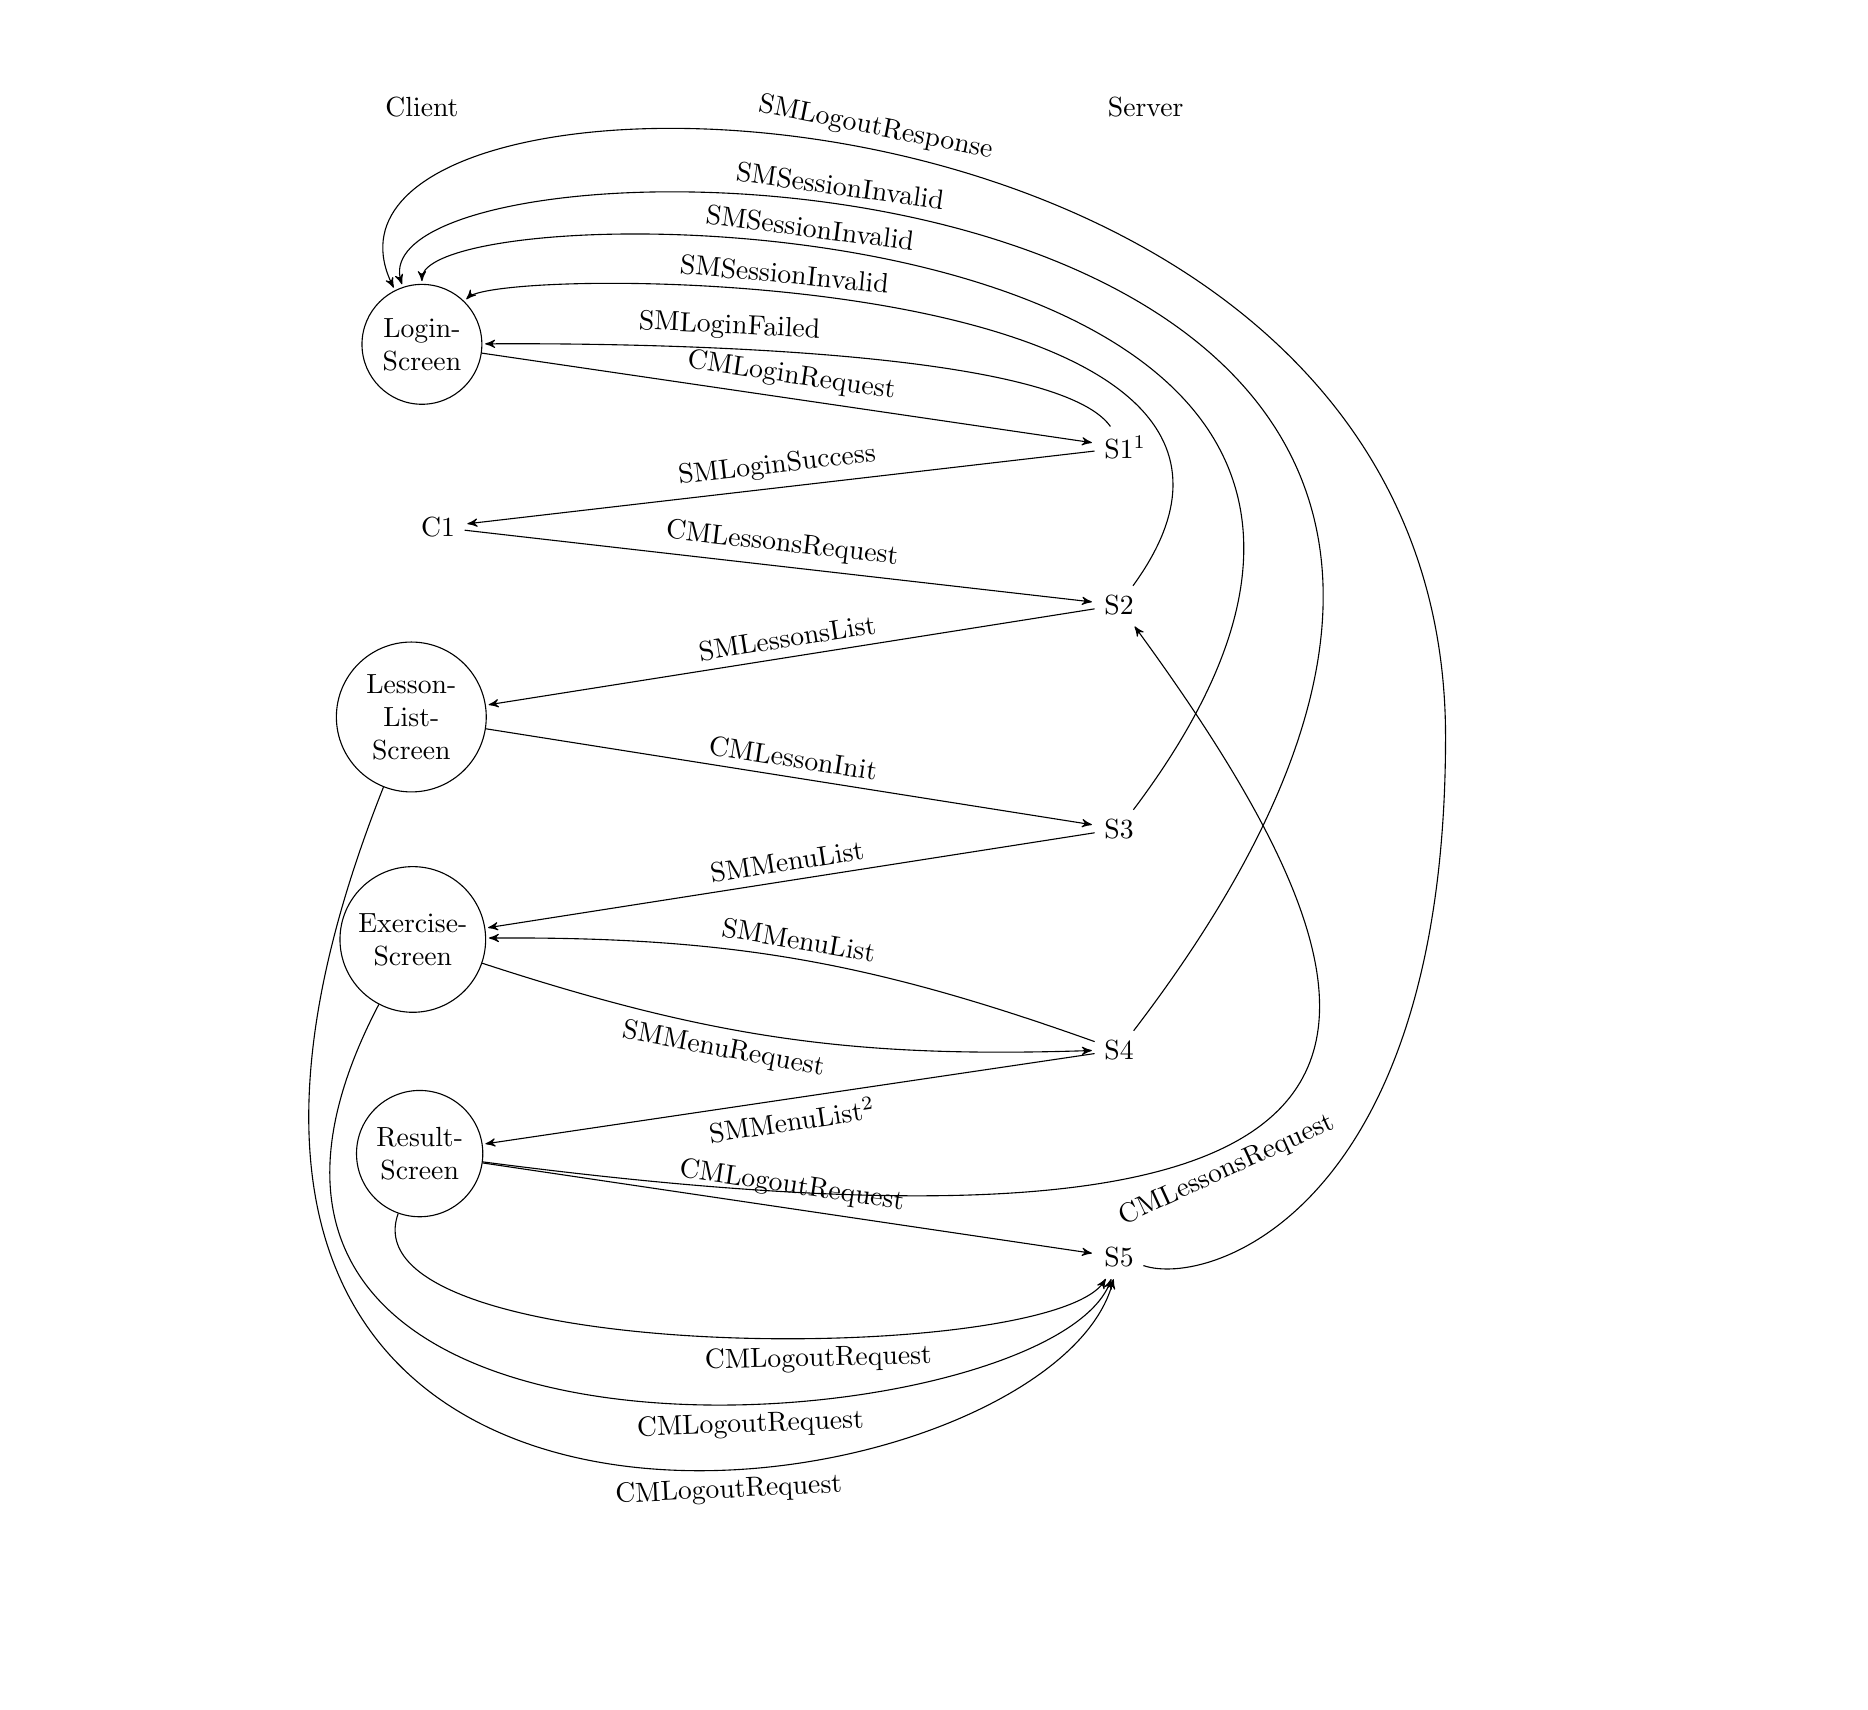
\begin{tikzpicture}[->,>=stealth',shorten >=1pt,auto]
    %\draw[help lines] (0,0) grid (15,-20);
    \node (client) {Client} ;
    \node (server) [right=8cm of client] {Server} ;
    \node[draw,circle,align=center] (login) [below=2cm of client] {Login-\\ Screen} ;
    \node (s1) [below right=0.5cm and 8cm of login] {S1\footnote{S1,..,S5,C1 are hidden states}} ;
    \node (c1) [below left=0.5cm and 8cm of s1] {C1} ;
    \node (s2) [below right=0.5cm and 8cm of c1] {S2} ;
    \node[draw,circle,align=center] (lesson) [below left=0.5cm and 8cm of s2] {Lesson-\\ List-\\ Screen} ;
    \node (s3) [below right=0.5cm and 8cm of lesson] {S3} ;
    \node[draw,circle,align=center] (exercise) [below left=0.5cm and 8cm of s3] {Exercise-\\ Screen} ;
    \node (s4) [below right=0.5cm and 8cm of exercise] {S4} ;
    \node[draw,circle,align=center] (result) [below left=0.5cm and 8cm of s4] {Result-\\ Screen} ;
    \node (s5) [below right=0.5cm and 8cm of result] {S5} ;
    \path
    (login) edge [sloped]node {CMLoginRequest} (s1)
    (s1) edge node [sloped] {SMLoginSuccess} (c1)
    (c1) edge node [sloped] {CMLessonsRequest} (s2) 
    (s2) edge node [sloped] {SMLessonsList} (lesson)
    (lesson) edge node [sloped] {CMLessonInit} (s3)
    (s3) edge node [above,sloped] {SMMenuList} (exercise)
    (exercise) edge [bend right=10] node [below,pos=0.4,sloped]{SMMenuRequest} (s4)
    (s4) edge [bend right=10] node [above,sloped] {SMMenuList} (exercise)
    (s4) edge node [below,sloped] {SMMenuList\footnote{If session is passed i.e. if both trees are the same}} (result)
    (result) edge node [sloped] {CMLogoutRequest} (s5);
    %\fill[fill=red] (-6,-20) circle [radius=2pt];
    %% \fill[fill=red] (-2,1) circle [radius=2pt];
    \draw[->] (s1) .. controls (8,-3) and (2,-3) .. (login) node [above,sloped,midway,pos=0.6] {SMLoginFailed} ;
    \draw[->] (s2) .. controls (12,-2) and (1,-2) .. (login) node [above,sloped,midway,pos=0.6] {SMSessionInvalid} ;
    \draw[->] (s3) .. controls (15,-1) and (0,-1) .. (login) node [above,sloped,midway,pos=0.6] {SMSessionInvalid} ;
    \draw[->] (s4) .. controls (18,0) and (-1,0) .. (login) node [above,sloped,midway,pos=0.6] {SMSessionInvalid} ;
    \draw[->] (result) .. controls (13,-15) and (13,-12) .. (s2) node [below,sloped,pos=0.4] {CMLessonsRequest} ;
    \draw[->] (s5) .. controls (10,-15) and (13,-14) .. (13,-8) .. controls (13,1) and (-2,1) .. (login) node [above,sloped,midway,pos=0.5] {SMLogoutResponse} ;
    \draw[->] (lesson) .. controls (-5,-20) and (8,-18) .. (s5) node [below,sloped,pos=0.6] {CMLogoutRequest} ;
    \draw[->] (exercise) .. controls (-4,-18) and (8,-17) .. (s5) node [below,sloped,pos=0.6] {CMLogoutRequest} ;
    \draw[->] (result) .. controls (-1,-16) and (8,-16) .. (s5) node [below,sloped,pos=0.6] {CMLogoutRequest} ;
  \end{tikzpicture}
\end{minipage}

\section{Database}

\subsection{ER-Diagram}

\tikzset{
  entity/.style={
    draw,
    rectangle
  },
  weak/.style={
    draw,
    rectangle,
    double
  },
  attribute/.style={
    draw,
    ellipse
  },
  relationship/.style={
    draw,
    diamond,
    aspect=1.6
  },
  supporting/.style={
    draw,
    diamond,
    aspect=1.6,
    double
  }
}
\resizebox{\textwidth}{!}{
\begin{tikzpicture}
  \node[entity] (user) {User} ;
  \node[attribute] (userUsername) [above left=1cm and 2cm of user] {\underline{Username}} ;
  \node[attribute] (userPassword) [above=1cm of user] {Password} ;
  \node[attribute] (userSalt) [above right= 1cm and 2cm of user] {Salt} ;
  \node[entity] (session) at (7,-5) {Session} ;
  \node[attribute] (sessionToken) [above left=1cm and 1cm of session] {\underline{Token}} ;
  \node[attribute] (sessionStarttime) [below=1cm of session] {Starttime} ;
  \node[attribute] (sessionLastActive) [above right=1cm and 1cm of session] {LastActive} ;
  \node[entity] (lesson) [below=5cm of user] {Lesson} ;
  \node[attribute] (lessonName) [below right=0.5cm and 0.5cm of lesson] {\underline{Name}} ;
  \node[attribute] (lessonGrammar) [left=1cm of lesson] {Grammar} ;
  \node[attribute] (lessonDescription) [below left=1cm and 1cm of lesson] {Description} ;
  \node[attribute] (lessonSourceLanguage) [below left=3cm and 1cm of lesson] {SourceLanguage} ;
  \node[attribute] (lessonTargetLanguage) [below right=3cm and 1cm of lesson] {TargetLanguage} ;
  \node[attribute] (lessonExerciseCount) [above left=1cm and 1cm of lesson] {ExerciseCount} ;
  \node[weak] (exercise) [below=5cm of lesson] {Exercise} ;
  \node[attribute] (exerciseSourceTree) [below left=1cm and 1cm of exercise] {\underline{SourceTree}};
  \node[attribute] (exerciseTargetTree) [below right=1cm and 1cm of exercise] {\underline{TargetTree}};
  \node[relationship] (takes) [below left=2cm and 1cm of user] {takes} ;
%  \node[attribute] (takesProgress) [above left=1cm and 1cm of takes] {Progress} ;
  \node[relationship] (lessonFinished) [below =2cm of user] {finished} ;
  \node[attribute] (lessonFinishedTime) [below right=1cm and 1cm of lessonFinished] {Time} ;
  \node[relationship] (usedBy) at (7,0) {usedBy} ;
  \node[supporting] (definedIn) [below=2cm of lesson] {definedIn} ;
  \node[relationship] (exerciseFinished) at (-7,-5) {finished} ;
  \node[attribute] (exerciseFinishedTime) [above right=1cm and 1cm of exerciseFinished] {Time} ;
  \node[relationship] (lessonUserExerciseList) [right=1.5cm of lesson] {exerciseInLesson};
  \path
  % User attributes
  (user) edge (userUsername)
  (user) edge (userPassword)
  (user) edge (userSalt)
  % Session attributes
  (session) edge (sessionToken)
  (session) edge (sessionLastActive)
  (session) edge (sessionStarttime)
  % Lesson attributes
  (lesson) edge (lessonName)
  (lesson) edge (lessonDescription)
  (lesson) edge (lessonGrammar)
  (lesson) edge (lessonExerciseCount)
  (lesson) edge (lessonSourceLanguage)
  (lesson) edge (lessonTargetLanguage)
  % Exercise attributed
  (exercise) edge (exerciseSourceTree)
  (exercise) edge (exerciseTargetTree)
  % takes relationship
  (user) edge (takes)
  (takes) edge (lesson)
  % takes attributes
%  (takes) edge (takesProgress)
  % finished relationship
  (user) edge (lessonFinished)
  (lessonFinished) edge (lesson)
  % finished attributes
  (lessonFinished) edge (lessonFinishedTime)
  % uses relationship
  (user) edge[(-] (usedBy)
  (usedBy) edge (session)
  % definedIn relationshio
  (lesson) edge[(-] (definedIn)
  (definedIn) edge (exercise)
  % exerciseFinished attributes
  (exerciseFinished) edge (exerciseFinishedTime)
  % lessonUserExerciseList
  (user) edge (lessonUserExerciseList)
  (lesson) edge (lessonUserExerciseList)
  (lessonUserExerciseList) edge (exercise)
  ;
  \draw (user) -- (-7,0) -- (exerciseFinished) ;
  \draw (exercise) -- (-7,-11) -- (exerciseFinished) ;
\end{tikzpicture}
}

\subsection{Schema}
\begin{description}
\item User(\underline{Username},Password,Salt)
\item Session(\underline{Token},User,Starttime,LastActive)
  \begin{description}
  \item User $\rightarrow$ User.Username
  \end{description}
\item Lesson(\underline{Name},Description,Grammar,SourceLanguage,TargetLanguage,ExerciseCount)
\item Exercise(\underline{SourceTree},\underline{TargetTree},\underline{Lesson})
  \begin{description}
  \item Lesson $\rightarrow$ Lesson.Name
  \end{description}
\item FinishedExercise(\underline{User},\underline{SourceTree},\underline{TargetTree},\underline{Lesson},Time,ClickCount)
  \begin{description}
  \item User $\rightarrow$ User.Username
  \item (SourceTree,TargetTree,Lesson) $\rightarrow$ Exercise.(SourceTree,TargetTree,Lesson)
  \end{description}
\item StartedLesson(\underline{Lesson},\underline{User})
  \begin{description}
  \item User $\rightarrow$ User.Username
  \item Lesson $\rightarrow$ Lesson.Name
  \end{description}
\item FinishedLesson(\underline{Lesson},\underline{User},Time)
  \begin{description}
  \item User $\rightarrow$ User.Username
  \item Lesson $\rightarrow$ Lesson.Name
  \end{description}
\item ExerciseList(\underline{User},\underline{SourceTree},\underline{TargetTree},\underline{Lesson})
  \begin{description}
  \item User $\rightarrow$ User.Username
  \item (SourceTree,TargetTree,Lesson) $\rightarrow$ Exercise.(SourceTree,TargetTree,Lesson)
  \item Lesson $\rightarrow$ Lesson.Name
  \end{description}
\end{description}

\subsection{SQLite SQL}

\begin{lstlisting}[language=SQL]
  CREATE TABLE User (
    Username TEXT,
    Password BLOB,
    Salt BLOB,
     PRIMARY KEY(Username)
    );
  CREATE TABLE Session (
    Token TEXT,
    Starttime NUMERIC DEFAULT CURRENT_TIMESTAMP,
    LastActive NUMERIC DEFAULT CURRENT_TIMESTAMP,
    PRIMARY KEY(Token)
    );
  CREATE TABLE Lesson (
    Name TEXT,
    Description TEXT,
    Grammar TEXT,
    SourceLanguage TEXT,
    TargetLanguage TEXT,
    ExerciseCount NUMERIC,
    PRIMARY KEY(Name)
    );
  CREATE TABLE Exercise (
    SourceTree TEXT,
    TargetTree TEXT,
    Lesson TEXT,
    PRIMARY KEY(SourceTree, TargetTree, Lesson),
    FOREIGN KEY(Lesson) REFERENCES Lesson(Name)
    );
  CREATE TABLE FinishedExercise(
    User TEXT,
    SourceTree TEXT,
    TargetTree TEXT,
    Lesson TEXT,
    Time NUMERIC,
    ClickCount NUMERIC,
    PRIMARY KEY(User,SourceTree,TargetTree,Lesson),
    FOREIGN KEY(User) REFERENCES User(Username),
    FOREIGN KEY(SourceTree,TargetTree,Lesson) REFERENCES Exercis(SourceTree,TargetTree,Lesson)
    );
  CREATE TABLE StartedLesson (
    Lesson TEXT,
    User TEXT,
    PRIMARY KEY(Lesson,User),
    FOREIGN KEY(Lesson) REFERENCES Lesson(Name),
    FOREIGN KEY(User) REFERENCES User(Username)
    );
  CREATE TABLE FinishedLesson(
    Lesson TEXT,
    User TEXT,
    Time NUMERIC,
    FOREIGN KEY (User) REFERENCES User(Username),
    FOREIGN KEY (Lesson) REFERENCES Lesson(Name)
    );
  CREATE TABLE ExerciseList(
    User TEXT,
    SourceTree TEXT,
    TargetTree TEXT,
    Lesson TEXT,
    PRIMARY KEY(User,SourceTree,TargetTree,Lesson),
    FOREIGN KEY(User) REFERENCES User(Username)
    FOREIGN KEY(SourceTree,TargetTree,Lesson) REFERENCES Exercise(SourceTree,TargetTree,Lesson)
    );
\end{lstlisting}

\end{document}
